\documentclass[dvips, lscape]{foils}
%\documentclass[dvips, french]{slides}
\textwidth 18.5cm
\textheight 25cm 
\topmargin -1cm 
\oddsidemargin  -1cm 
\evensidemargin  -1cm

% Maths
\usepackage{amsfonts, amsmath, amssymb}

\newcommand{\coefbin}[2]{\left( 
    \begin{array}{c} #1 \\ #2 \end{array} 
  \right)}
\newcommand{\bbullet}{\bullet\bullet}
\newcommand{\bbbullet}{\bbullet\bullet}
\newcommand{\bbbbullet}{\bbbullet\bullet}
\newcommand{\Bcal}{\mathcal{B}}
\newcommand{\Ccal}{\mathcal{C}}
\newcommand{\Dcal}{\mathcal{D}}
\newcommand{\Ecal}{\mathcal{E}}
\newcommand{\Mcal}{\mathcal{M}}
\newcommand{\Ncal}{\mathcal{N}}
\newcommand{\Pcal}{\mathcal{P}}
\newcommand{\Qcal}{\mathcal{Q}}
\newcommand{\Lcal}{\mathcal{L}}
\newcommand{\Tcal}{\mathcal{T}}
\newcommand{\Ucal}{\mathcal{U}}
\newcommand{\Xcal}{\mathcal{X}}
\newcommand{\Zcal}{\mathcal{Z}}
\newcommand{\etabar}{\overline{\eta}}
\newcommand{\pibar}{\overline{\pi}}
\newcommand{\alphabf}{\mbox{\mathversion{bold}{$\alpha$}}}
\newcommand{\betabf}{\mbox{\mathversion{bold}{$\beta$}}}
\newcommand{\gammabf}{\mbox{\mathversion{bold}\newcommand{\psibf}{\mbox{\mathversion{bold}{$\psi$}}}
{$\gamma$}}}
\newcommand{\mubf}{\mbox{\mathversion{bold}{$\mu$}}}
\newcommand{\psibf}{\mbox{\mathversion{bold}{$\psi$}}}
\newcommand{\Sigmabf}{\mbox{\mathversion{bold}{$\Sigma$}}}
\newcommand{\taubf}{\mbox{\mathversion{bold}{$\tau$}}}
\newcommand{\thetabf}{\mbox{\mathversion{bold}{$\theta$}}}
\newcommand{\Abf}{{\bf A}}
\newcommand{\Ebf}{{\bf E}}
\newcommand{\Hbf}{{\bf H}}
\newcommand{\Ibf}{{\bf I}}
\newcommand{\Sbf}{{\bf S}}
\newcommand{\mbf}{{\bf m}}
\newcommand{\ubf}{{\bf u}}
\newcommand{\vbf}{{\bf v}}
\newcommand{\xbf}{{\bf x}}
\newcommand{\Xbf}{{\bf X}}
\newcommand{\Esp}{{\mathbb E}}
\newcommand{\Corr}{{\mathbb C}\mbox{orr}}
\newcommand{\Var}{{\mathbb V}}
\newcommand{\Ibb}{{\mathbb I}}
\newcommand{\Rbb}{\mathbb{R}}
\newcommand{\Vsf}{\mathsf{V}}

% Couleur et graphiques
\usepackage{color}
\usepackage{graphics}
\usepackage{epsfig} 
\usepackage{pstcol}

% Texte
\usepackage{lscape}
\usepackage{../../../../Latex/fancyheadings, rotating, enumerate}
%\usepackage[french]{babel}
\usepackage[latin1]{inputenc}
%\definecolor{darkgreen}{cmyk}{0.5, 0, 0.5, 0.5}
%\definecolor{green}{cmyk}{0.5, 0, 0.5, 0.5}
\definecolor{orange}{cmyk}{0, 0.6, 0.8, 0}
\definecolor{jaune}{cmyk}{0, 0.5, 0.5, 0}
\newcommand{\textblue}[1]{\textcolor{blue}{#1}}
\newcommand{\textred}[1]{\textcolor{red}{#1}}
\newcommand{\textgreen}[1]{\textcolor{green}{ #1}}
\newcommand{\textlightgreen}[1]{\textcolor{green}{#1}}
%\newcommand{\textgreen}[1]{\textcolor{darkgreen}{#1}}
\newcommand{\textorange}[1]{\textcolor{orange}{#1}}
\newcommand{\textyellow}[1]{\textcolor{yellow}{#1}}
\newcommand{\refer}[2]{{\sl #1}}

% Sections
%\newcommand{\chapter}[1]{\centerline{\LARGE \textblue{#1}}}
% \newcommand{\section}[1]{\centerline{\Large \textblue{#1}}}
% \newcommand{\subsection}[1]{\noindent{\Large \textblue{#1}}}
% \newcommand{\subsubsection}[1]{\noindent{\large \textblue{#1}}}
% \newcommand{\paragraph}[1]{\noindent {\textblue{#1}}}
% Sectionsred
\newcommand{\chapter}[1]{
  \addtocounter{chapter}{1}
  \setcounter{section}{0}
  \setcounter{subsection}{0}
%  {\centerline{\LARGE \textblue{\arabic{chapter} - #1}}}
  {\centerline{\LARGE \textblue{#1}}}
  }
\newcommand{\section}[1]{
  \addtocounter{section}{1}
  \setcounter{subsection}{0}
%  {\centerline{\Large \textblue{\arabic{chapter}.\arabic{section} - #1}}}
  {\centerline{\Large \textblue{#1}}}
  }
\newcommand{\subsection}[1]{
  \addtocounter{subsection}{1}
%  {\noindent{\large \textblue{\arabic{chapter}.\arabic{section}.\arabic{subsection} - #1}}}
  {\noindent{\large \textblue{#1}}}
  }
\newcommand{\paragraph}[1]{\noindent{\textblue{#1}}}

%%%%%%%%%%%%%%%%%%%%%%%%%%%%%%%%%%%%%%%%%%%%%%%%%%%%%%%%%%%%%%%%%%%%%%
%%%%%%%%%%%%%%%%%%%%%%%%%%%%%%%%%%%%%%%%%%%%%%%%%%%%%%%%%%%%%%%%%%%%%%
%%%%%%%%%%%%%%%%%%%%%%%%%%%%%%%%%%%%%%%%%%%%%%%%%%%%%%%%%%%%%%%%%%%%%%
%%%%%%%%%%%%%%%%%%%%%%%%%%%%%%%%%%%%%%%%%%%%%%%%%%%%%%%%%%%%%%%%%%%%%%
\begin{document}
%%%%%%%%%%%%%%%%%%%%%%%%%%%%%%%%%%%%%%%%%%%%%%%%%%%%%%%%%%%%%%%%%%%%%%
%%%%%%%%%%%%%%%%%%%%%%%%%%%%%%%%%%%%%%%%%%%%%%%%%%%%%%%%%%%%%%%%%%%%%%
%%%%%%%%%%%%%%%%%%%%%%%%%%%%%%%%%%%%%%%%%%%%%%%%%%%%%%%%%%%%%%%%%%%%%%
%%%%%%%%%%%%%%%%%%%%%%%%%%%%%%%%%%%%%%%%%%%%%%%%%%%%%%%%%%%%%%%%%%%%%%
\landscape
\newcounter{chapter}
\newcounter{section}
\newcounter{subsection}
\setcounter{chapter}{0}
\headrulewidth 0pt 
\pagestyle{fancy} 
\cfoot{}
\rfoot{\begin{rotate}{90}{
      \hspace{1cm} \tiny S. Robin: A mixture model for random graphs 
      }\end{rotate}}
\rhead{\begin{rotate}{90}{
      \hspace{-.5cm} \tiny \thepage
      }\end{rotate}}

%%%%%%%%%%%%%%%%%%%%%%%%%%%%%%%%%%%%%%%%%%%%%%%%%%%%%%%%%%%%%%%%%%%%%%
%%%%%%%%%%%%%%%%%%%%%%%%%%%%%%%%%%%%%%%%%%%%%%%%%%%%%%%%%%%%%%%%%%%%%%
\begin{center}
  \textblue{\LARGE A mixture model for random graphs} 

   \vspace{1cm}
   {\large J-J Daudin, F. Picard, S. Robin} \\
   robin@inapg.inra.fr

   {UMR INA-PG / ENGREF / INRA, Paris} \\
   {Math�matique et Informatique Appliqu�es}
   
\end{center}

\paragraph{Working group:} E. Birmele, C. Matias, F. Muri (Evry
   univ.), S. Schbath (INRA-MIG)

\vspace{1cm}

\subsection{Data = biological network} \\
Protein interaction network, reaction network, enzyme network, {\it etc.}

\subsection{Problem: Find groups of vertices} \\
Groups of proteins, reactions, enzymes according to the connections
between them.

% \vspace{2cm}
% \paragraph{Examples of random networks.} 
% $$
% \begin{tabular}{ll}
%   Social: & who knows who? \\
%   \\
%   Biological: & which protein interacts with which? \\
%   \\
%   Internet: & connection between servers or web pages.
% \end{tabular}
% $$

%%%%%%%%%%%%%%%%%%%%%%%%%%%%%%%%%%%%%%%%%%%%%%%%%%%%%%%%%%%%%%%%%%%%%
%%%%%%%%%%%%%%%%%%%%%%%%%%%%%%%%%%%%%%%%%%%%%%%%%%%%%%%%%%%%%%%%%%%%%
\newpage
\chapter{Random graphs}
%%%%%%%%%%%%%%%%%%%%%%%%%%%%%%%%%%%%%%%%%%%%%%%%%%%%%%%%%%%%%%%%%%%%%

\paragraph{Notation and definition.} Given a set of $n$ vertices ($i = 1..n$),
$X_{ij}$ indicates the presence/absence of a (non oriented) edge
between vertices $i$ and $j$:
$$
X_{ij} = X_{ji} = \left\{ 
  \begin{array}{rl}
    1 & \mbox{if } i \leftrightarrow j, \\
    0 & \mbox{otherwise}
  \end{array} \right.
\qquad X_{ii} = 0.
$$
The random graph is defined by the join distribution of all the
$\{X_{ij}\}_{i, j}$.

\vspace{1cm}
\paragraph{Typical characteristics.} 

\noindent\begin{tabular}{ll}
  Degree (connectivity) of the vertices: & ${K_i = \sum_{j
      \neq i} X_{ij}}$ \\
  \\
  Clustering coefficient: &  ${c = \Pr\{X_{jk} = 1 \;|\;
    X_{ij} = X_{ik} = 1 \}}$ \\
  \\
  Diameter: & Longest path between two vertices.
\end{tabular}

%%%%%%%%%%%%%%%%%%%%%%%%%%%%%%%%%%%%%%%%%%%%%%%%%%%%%%%%%%%%%%%%%%%%%
\newpage
\subsection{Erdos-R�nyi (ER) model}

\paragraph{Definition.} The $\{X_{ij}\}_{i, j}$ are i.i.d.: 
$$
X_{ij} \sim \Bcal(p).  
$$

\paragraph{Characteristics.}

\noindent\begin{tabular}{ll}
  Degree : & $K_i \sim \Bcal(n-1, p) \approx \Pcal(\lambda)$ \\
  \\
  Clustering coefficient: &  ${c = p}$ \\
\end{tabular}


\vspace{1cm}
\paragraph{Drawback.} The ER fits poorly many real-world networks.
\begin{itemize}
\item Empirical degree distributions are often very different from the
  Poisson distribution because of few vertices having very high
  degrees.
\item Empirical clustering coefficients are generally higher than
  expected under ER.
\end{itemize}

%%%%%%%%%%%%%%%%%%%%%%%%%%%%%%%%%%%%%%%%%%%%%%%%%%%%%%%%%%%%%%%%%%%%%
\newpage
\chapter{Mixture model for the degrees} \label{Sec:PoissonMixture}
%%%%%%%%%%%%%%%%%%%%%%%%%%%%%%%%%%%%%%%%%%%%%%%%%%%%%%%%%%%%%%%%%%%%%

\paragraph{Scale-free distribution.} The most popular alternative to
the Poisson distribution is the Zipf distribution:
$$
\Pr\{K = k\} = c(\rho)k^{-(\rho+1)},
$$
where $\rho > 0$ and $c(\rho)$ is a normalizing constant. (Not
defined for $k = 0$.)

\bigskip\bigskip
\paragraph{Mixture model.} We propose to generalize the ER model
assuming that the vertices belong to $Q$ different groups with
different mean degrees. 

We denote $\alpha_q$ the prior probability (proportion) of each group
$$
\alpha_q = \Pr\{i \in q\}, 
\quad 
\sum_q \alpha_q = 1
$$
and $Z_{iq}$ the binary variable indicating if vertex $i$ belongs
to group $q$:
$
Z_{iq} = \Ibb\{i \in q\}.
$

%%%%%%%%%%%%%%%%%%%%%%%%%%%%%%%%%%%%%%%%%%%%%%%%%%%%%%%%%%%%%%%%%%%%%
\newpage
\paragraph{Distribution of the degrees.} $K$ has a mixture
distribution
$$
K \sim \sum_q \alpha_q \Pcal(\lambda_q)
\qquad \Rightarrow \qquad
\Pr \{ K = k \}= \sum_{q=1}^Q \alpha_q \frac{e^{-\lambda_q} \lambda_q^k}{k!}.
$$

%%%%%%%%%%%%%%%%%%%%%%%%%%%%%%%%%%%%%%%%%%%%%%%%%%%%%%%%%%%%%%%%%%%%%
\subsection{Application to {\it E. coli} reaction network}

\begin{itemize}
\item \vspace{-0.5cm} $n = 605$ vertices (reactions) and $1\;782$
  edges. 
\item \vspace{-0.5cm} 2 reactions $i$ and $j$ are connected if the
  product of $i$ is the substrate of $j$ (or conversely).
\item \vspace{-0.5cm} provided by V. Lacroix and M.-F. Sagot (INRIA
H�lix).
\end{itemize}

\paragraph{Parameter estimates.} The BIC criterion select $Q = 3$ groups:
$$
\begin{tabular}{cccc}
  group & 1 & 2 & 3 \\
  \hline
  $\widehat{\alpha}$ (\%) & 8.9 & 19.7 & 71.3 \\
  $\widehat{\lambda}$ & 21.5 & 9.1 & 3.0 \\
\end{tabular}
$$

%%%%%%%%%%%%%%%%%%%%%%%%%%%%%%%%%%%%%%%%%%%%%%%%%%%%%%%%%%%%%%%%%%%%%
\newpage
\paragraph{Distribution fits.} 
$$
\begin{tabular}{cccc}
  Distribution & \begin{tabular}{c}log-log plot \\ / histogram
  \end{tabular} & \multicolumn{2}{c}{P-P plot} \\ 
%  \\
  \hline
  \begin{tabular}{c} Zipf \end{tabular}
  & \begin{tabular}{c} \epsfig{file = ../figures/log_log.eps,
      height=5cm, width = 5cm} \end{tabular}
  & \begin{tabular}{c} \epsfig{file = ../figures/PPplot1.eps,
      height=5cm, width = 5cm} \end{tabular}
  & \begin{tabular}{c} \epsfig{file = ../figures/PPplot6.eps, height=5cm, width =
      5cm} \end{tabular} \\ 
  & & threshold = 1 & threshold = 6 \\
  \hline
%  \\
  \begin{tabular}{c} Poisson \\ mixture \end{tabular}
  & \begin{tabular}{c} 
    %\epsfig{file = ../figures/degre_melange.eps, height=5cm, width=5cm} 
    \epsfig{file = ../figures/ECOli-Poisson-Q3.eps, height=5cm,
    width=5cm, angle=90, bbllx=335, bblly=415, bburx=555, bbury=700, clip=}  
  \end{tabular}
  & \begin{tabular}{c} 
    %\epsfig{file = ../figures/PPplot_melange.eps, height=5cm, width=5cm} 
    \epsfig{file = ../figures/ECOli-Poisson-Q3.eps, height=5cm,
    width=5cm, angle=90, bbllx=65, bblly=80, bburx=285, bbury=360, clip=} 
  \end{tabular} \\
\end{tabular}
$$
%\paragraph{Preliminary conclusions.}
\begin{itemize}
\item \vspace{-0.5cm} The Poisson mixture fits the data well, better
  than the Zipf model.
\item \vspace{-0.5cm} But a model for the degrees is not a model for
  the graph.
\end{itemize}

% %%%%%%%%%%%%%%%%%%%%%%%%%%%%%%%%%%%%%%%%%%%%%%%%%%%%%%%%%%%%%%%%%%
% \newpage
% \paragraph{Distribution plots.} 
% $$
% \begin{tabular}{cccc}
%   Distribution & \begin{tabular}{c}log-log plot \\ / histogram
%   \end{tabular} & \multicolumn{2}{c}{P-P plot} \\ 
%  \\
%   \hline
%   \begin{tabular}{c} Zipf \end{tabular}
%   & \begin{tabular}{c} \epsfig{file = ../figures/log_log.eps,
%       height=5cm, width = 5cm} \end{tabular}
%   & \begin{tabular}{c} \epsfig{file = ../figures/PPplot1.eps,
%       height=5cm, width = 5cm} \end{tabular}
%   & \begin{tabular}{c} \epsfig{file = ../figures/PPplot6.eps, height=5cm, width =
%       5cm} \end{tabular} \\ 
%   & & threshold = 1 & threshold = 6 \\
%   \hline
%  \\
%   \begin{tabular}{c} Poisson \\ mixture \end{tabular}
%   & \begin{tabular}{c} 
%     %\epsfig{file = ../figures/degre_melange.eps, height=5cm, width=5cm} 
%     \epsfig{file = ../figures/ECOli-Poisson-Q3.eps, height=5cm,
%     width=5cm, angle=90, bbllx=335, bblly=415, bburx=555, bbury=700, clip=}  
%   \end{tabular}
%   & \begin{tabular}{c} 
%     %\epsfig{file = ../figures/PPplot_melange.eps, height=5cm, width=5cm} 
%     \epsfig{file = ../figures/ECOli-Poisson-Q3.eps, height=5cm,
%     width=5cm, angle=90, bbllx=65, bblly=80, bburx=285, bbury=360, clip=} 
%   \end{tabular} \\
% \end{tabular}
% $$

% %%%%%%%%%%%%%%%%%%%%%%%%%%%%%%%%%%%%%%%%%%%%%%%%%%%%%%%%%%%%%%%%%%
% \newpage
% \paragraph{Fit statistics.} The Zipf distribution is only defined
% above a certain threshold. 
% $$
% \begin{tabular}{ccccccccc}
%   & & \multicolumn{4}{c}{Power law} & \multicolumn{3}{c}{Poisson mixture} \\
%   Threshold & $n$ & $\rho+1$ & $\chi^2$ stat. & df & $p$-value
%   & $\chi^2$ stat. & df & $p$-value \\
%   \hline
%   0 & 593 & -    & -     & -  & -            & 67.25 & 29 & $7\;10^{-5}$\\
%   1 & 549 & 1.79 & 96.22 & 32 & $2\;10^{-9}$ & 58.5  & 28 & $6\;10^{-4}$\\
%   2 & 399 & 1.93 & 75.83 & 31 & $1\;10^{-6}$ & 32.3  & 27 & $0.22$\\
%   3 & 315 & 2.08 & 59.70 & 30 & $0.001     $ & 30.6  & 26 & $0.24$\\
%   4 & 252 & 2.19 & 53.07 & 29 & $0.004     $ & 27.0  & 25 & $0.36$\\
%   5 & 200 & 2.24 & 52.37 & 28 & $0.003     $ & 27.0  & 24 & $0.30$\\
%   6 & 172 & 2.37 & 45.44 & 27 & $0.014     $ & 25.0  & 23 & $0.35$\\
% \end{tabular}
% $$

% \paragraph{Preliminary conclusions.}
% \begin{itemize}
% \item \vspace{-0.5cm} The Poisson mixture fits the data well, better
%    than the Zipf model.
% \item \vspace{-0.5cm} But a model for the degrees is not a model for
%   the graph.
% \end{itemize}

%%%%%%%%%%%%%%%%%%%%%%%%%%%%%%%%%%%%%%%%%%%%%%%%%%%%%%%%%%%%%%%%%%%%%
%%%%%%%%%%%%%%%%%%%%%%%%%%%%%%%%%%%%%%%%%%%%%%%%%%%%%%%%%%%%%%%%%%%%%
\newpage
\chapter{Erd�s-R�nyi mixture for graph (ERMG)} \label{Sec:ErdosMixture}
%%%%%%%%%%%%%%%%%%%%%%%%%%%%%%%%%%%%%%%%%%%%%%%%%%%%%%%%%%%%%%%%%%%%%

%%%%%%%%%%%%%%%%%%%%%%%%%%%%%%%%%%%%%%%%%%%%%%%%%%%%%%%%%%%%%%%%%%%%%
\subsection{An explicit random graph model} 

\paragraph{Mixture population of edges.} We still suppose that the
edges belong to $Q$ groups:
$$
\alpha_q = \Pr\{i \in q\}, 
\qquad
Z_{iq} = \Ibb\{i \in q\}.
$$

\paragraph{Conditional distribution of the edges.}
The edges $\{X_{ij}\}$ are conditionally independent given the group of
the vertices:
$$
X_{ij} \; |\; \{i \in q, j \in \ell \} \sim \Bcal(\pi_{q\ell}).
$$
$\pi_{q\ell} = \pi_{\ell q}$ is the connection probability between
groups $q$ and $\ell$.

A high value of $\pi_{q\ell}$ reveals a preferential connectivity
between groups $q$ and $\ell$. 

% %%%%%%%%%%%%%%%%%%%%%%%%%%%%%%%%%%%%%%%%%%%%%%%%%%%%%%%%%%%%%%%%%%%%%
% \newpage
% \subsection{Some properties of the ERMG model}
% %%%%%%%%%%%%%%%%%%%%%%%%%%%%%%%%%%%%%%%%%%%%%%%%%%%%%%%%%%%%%%%%%%%%%

% \paragraph{Conditional distribution of the degrees:}
% $$
% K_i \;|\; \{i \in q \} \sim \Bcal(n-1, \pibar_q) \approx
% \Pcal(\lambda_q)
% $$
% where $ \pibar_q = \sum_{\ell} \alpha_{\ell} \pi_{q\ell}$,
% $\lambda_q = (n-1) \pibar_q$.

% \bigskip\bigskip
% \paragraph{Marginal distribution of the degrees:} we get a Poisson mixture
% $$
% K_i \sim \sum_q \Bcal(n-1, \pibar_q) \approx \sum_q \alpha_q \Pcal(\lambda_q).
% $$

% %%%%%%%%%%%%%%%%%%%%%%%%%%%%%%%%%%%%%%%%%%%%%%%%%%%%%%%%%%%%%%%%%%%%%
% \newpage
% \paragraph{Between-group connectivity.}
% $A_{q\ell}$ denotes the connectivity between groups $q$ and $\ell$:
% $$
% A_{q\ell} = \sum_{i<j} Z_{iq} Z_{j\ell} X_{ij}.
% $$
% In the ERMG model, its expectation is
% $$
% \Esp (A_{q\ell})  = \frac{n(n-1)}2 \alpha_q \alpha_{\ell} \pi_{q\ell}.
% $$

% \paragraph{Clustering coefficient:}  
% $$
% c = \Pr\{\nabla \cap \Vsf\} / \Pr\{\Vsf\} = \Pr\{\nabla\} /
% \Pr\{\Vsf\}.
% $$
% In the ERMG model, we get
% $$
% c = \frac{\sum_{q, \ell, m} \alpha_q \alpha_{\ell} \alpha_m \pi_{q\ell}
% \pi_{qm} \pi_{\ell m}}{\sum_{q, \ell, m} \alpha_q
%   \alpha_{\ell} \alpha_m \pi_{q\ell} \pi_{qm}}.
% $$

% %%%%%%%%%%%%%%%%%%%%%%%%%%%%%%%%%%%%%%%%%%%%%%%%%%%%%%%%%%%%%%%%%%%%%
% \newpage
% \subsection{Independent model}
% %%%%%%%%%%%%%%%%%%%%%%%%%%%%%%%%%%%%%%%%%%%%%%%%%%%%%%%%%%%%%%%%%%%%%

% The absence of preferential connection between groups corresponds to
% the case where
% $$
% \pi_{q\ell} = \eta_q \eta_{\ell}.
% $$

% \noindent
% \begin{tabular}{ll}
%   \paragraph{Distribution of degrees:} & $\{K_i \;|\; i \in q\} \sim
%   \Pcal(\lambda_q)$, \\
%   \\
%   & where \quad $\lambda_q = (n-1) \eta_q \etabar$, \quad $\etabar = \sum_{\ell}
%   \alpha_{\ell} \eta_{\ell}$. \\
%   \\
%   \paragraph{Between group connectivity:} & $\Esp (A_{q\ell}) = n(n-1)
%   (\alpha_q \eta_q) (\alpha_{\ell} \eta_{\ell}) / 2$. \\
%   \\
%   \paragraph{Clustering coefficient:} & $\displaystyle{c =  \frac{\left(\sum_q \alpha_q
%     \eta^2_q\right)^2}{\etabar^2}}$.
% \end{tabular}

% The ER model corresponds to 
% $$
% Q=1, \qquad \alpha_1=1, \qquad \etabar = \eta_1 = \sqrt{p},
% $$
% so we get the known result: $ c = \eta^4_1 / \eta^2_1 = p $.


%%%%%%%%%%%%%%%%%%%%%%%%%%%%%%%%%%%%%%%%%%%%%%%%%%%%%%%%%%%%%%%%%%%%%
\newpage
\subsection{Examples}
%%%%%%%%%%%%%%%%%%%%%%%%%%%%%%%%%%%%%%%%%%%%%%%%%%%%%%%%%%%%%%%%%%%%%
$$
\begin{tabular}{lcccc}
  Description & Network & $Q$ & $\pi$
  & \begin{tabular}{c} Clustering \\ coefficient \end{tabular}\\
  \hline
  \begin{tabular}{p{2cm}} Random \end{tabular}
  & \begin{tabular}{c}\epsfig{file = ../figures/FigNetworks-Erdos.eps, height=1.7cm,
      width=2.5cm, clip=, bbllx=120, bblly=260, bburx=530,
      bbury=570}  \end{tabular}
  & 1
  &  $p$ & $p$ \\
  \hline
  \begin{tabular}{p{2cm}} Independent model (product connectivity) \end{tabular}
  & \begin{tabular}{c}\epsfig{file = ../figures/FigNetworks-Indep.eps,
      height=2cm, width=4cm, clip=, bbllx=120, bblly=260, bburx=530,
      bbury=570}  \end{tabular}
  & 2
  & $\left( \begin{array}{cc} a^2 &ab\\ ab&b^2\\ \end{array}
  \right)$
  & $\displaystyle{\frac{(a^2+b^2)^2}{(a+b)^2}}$ \\
  \hline
  \begin{tabular}{p{2cm}} Stars \end{tabular}
  & \begin{tabular}{c}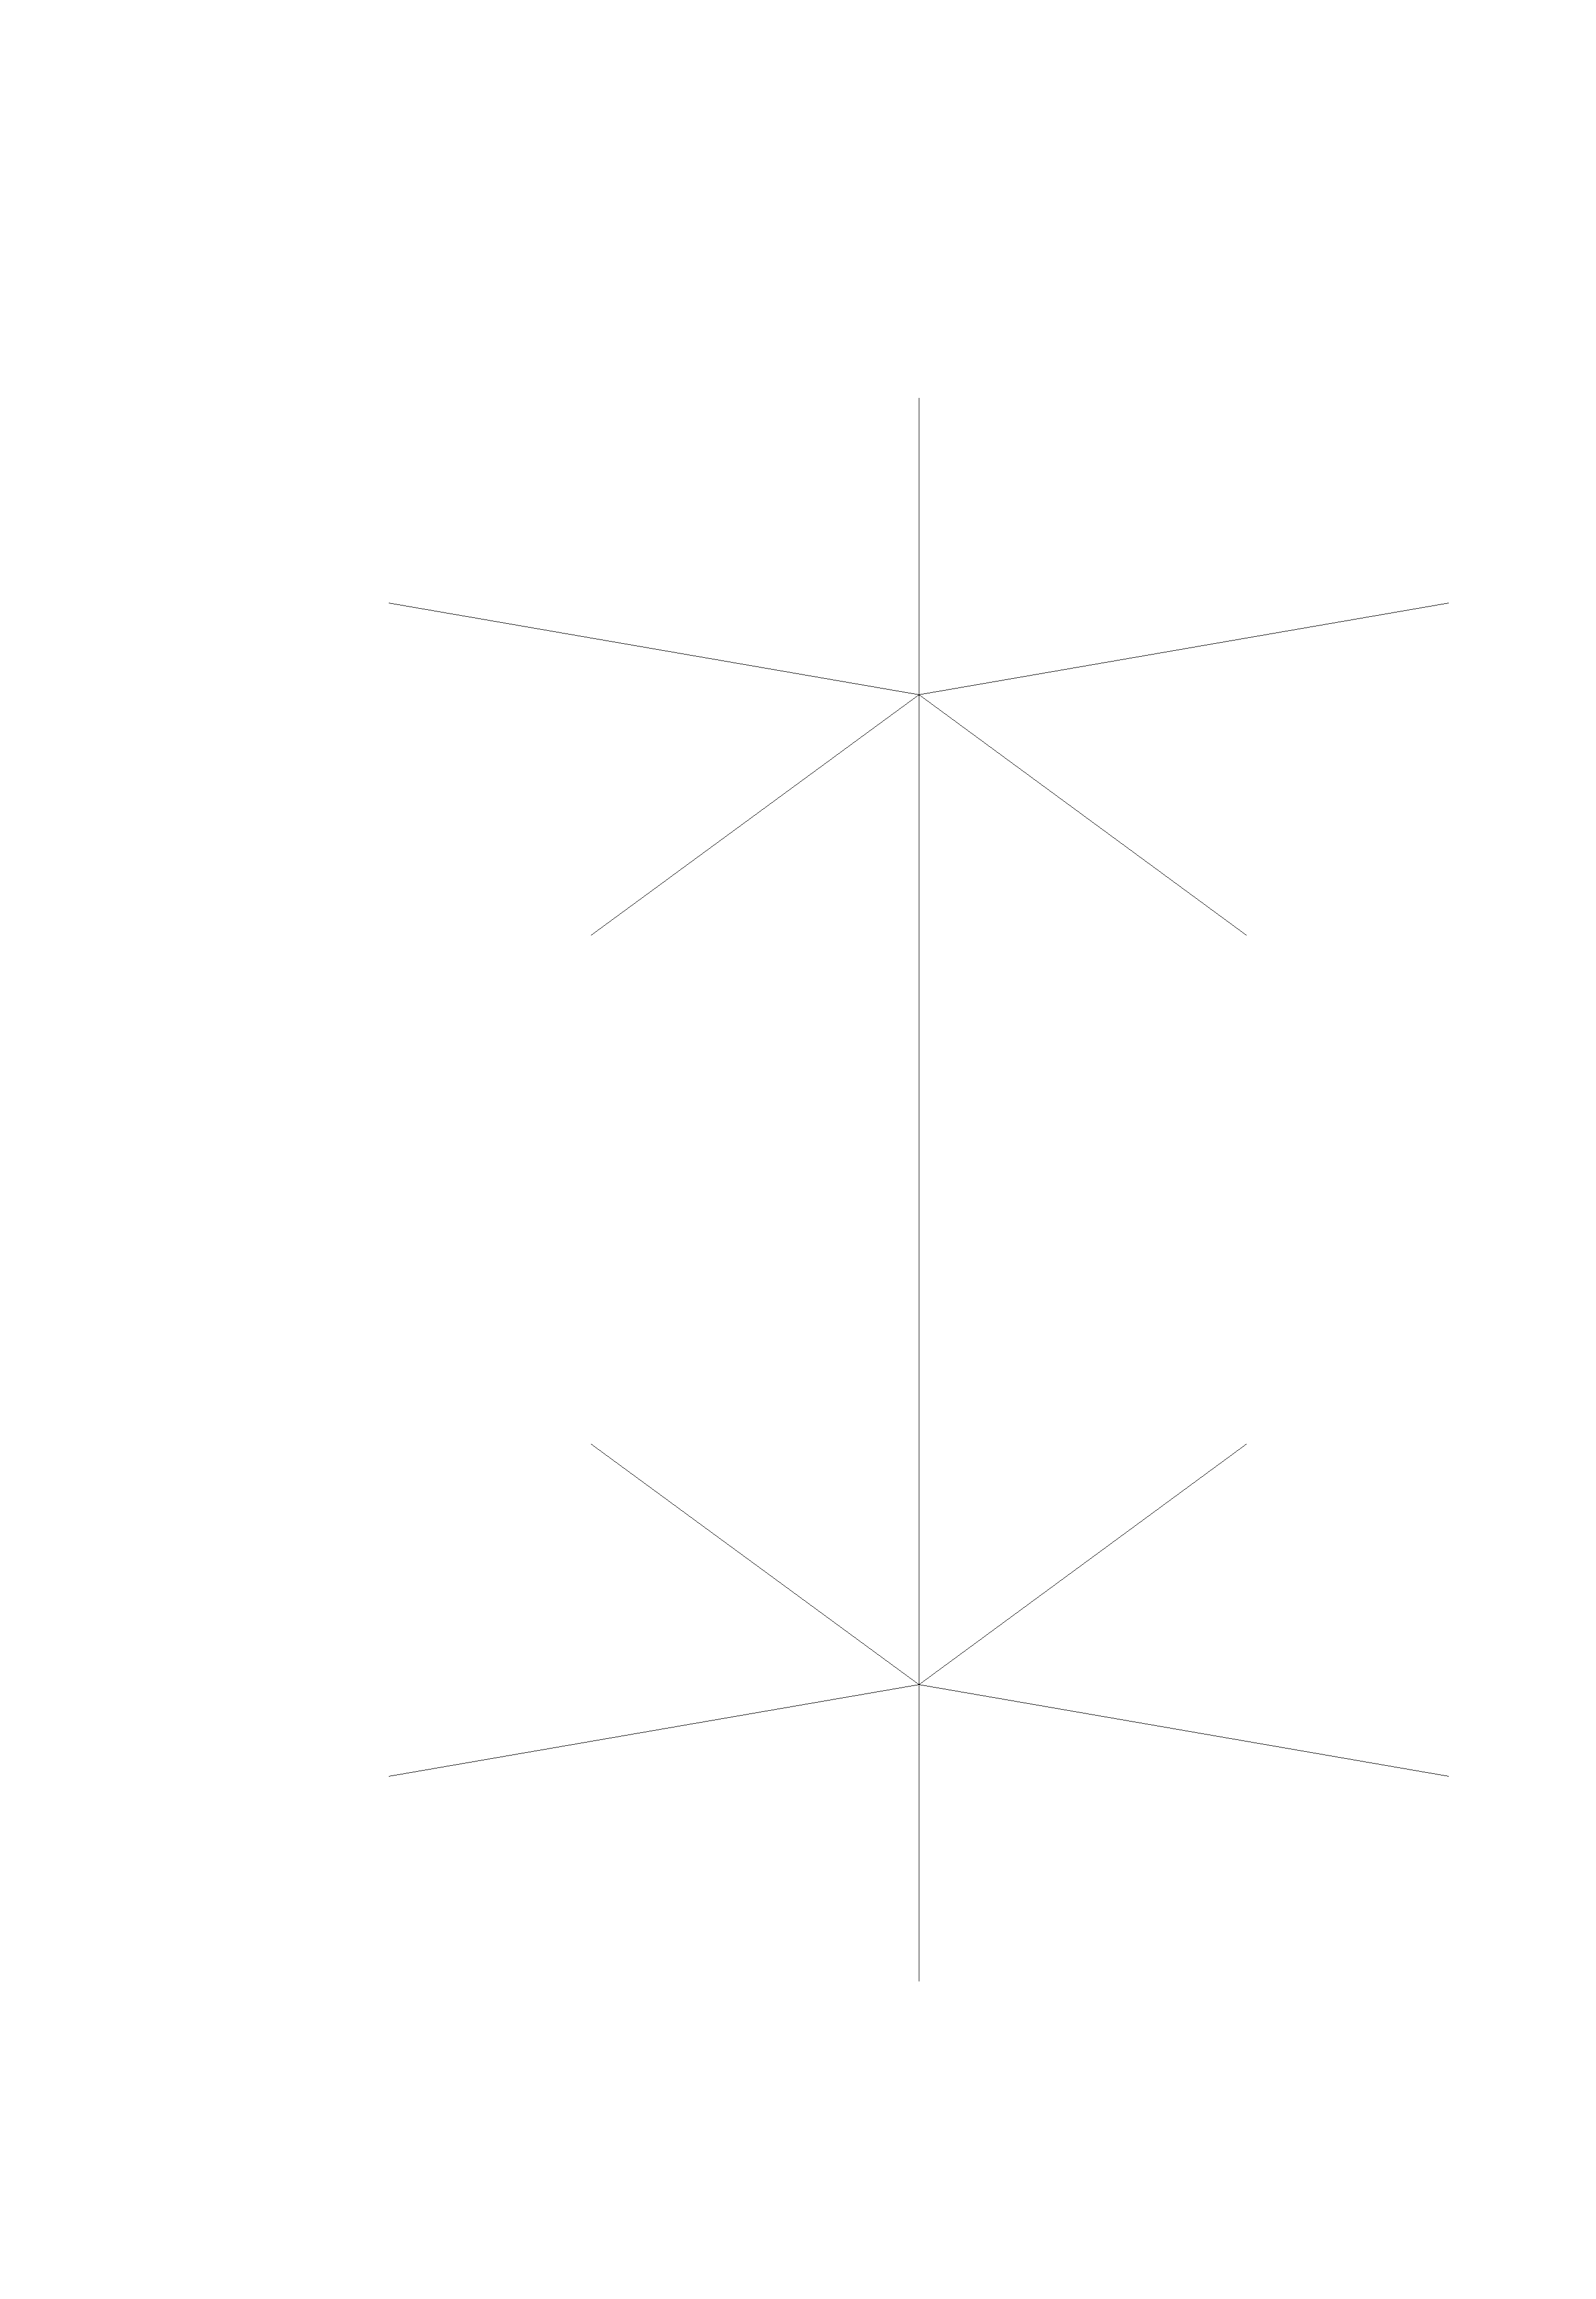
\epsfig{file = ../figures/FigNetworks-Star.eps, height=1.7cm,
      width=4cm, clip=, bbllx=120, bblly=260, bburx=530,
      bbury=570}   \end{tabular}
  & 4
  & $\left( \begin{array}{cccc} 0&1&0&0\\ 1&0&1&0\\0&1&0&1\\0&0&1&0\\
    \end{array} \right)$
  & 0 \\
  \hline \begin{tabular}{p{2cm}} Clusters (affiliation networks)
  \end{tabular}
  
  & \begin{tabular}{c} 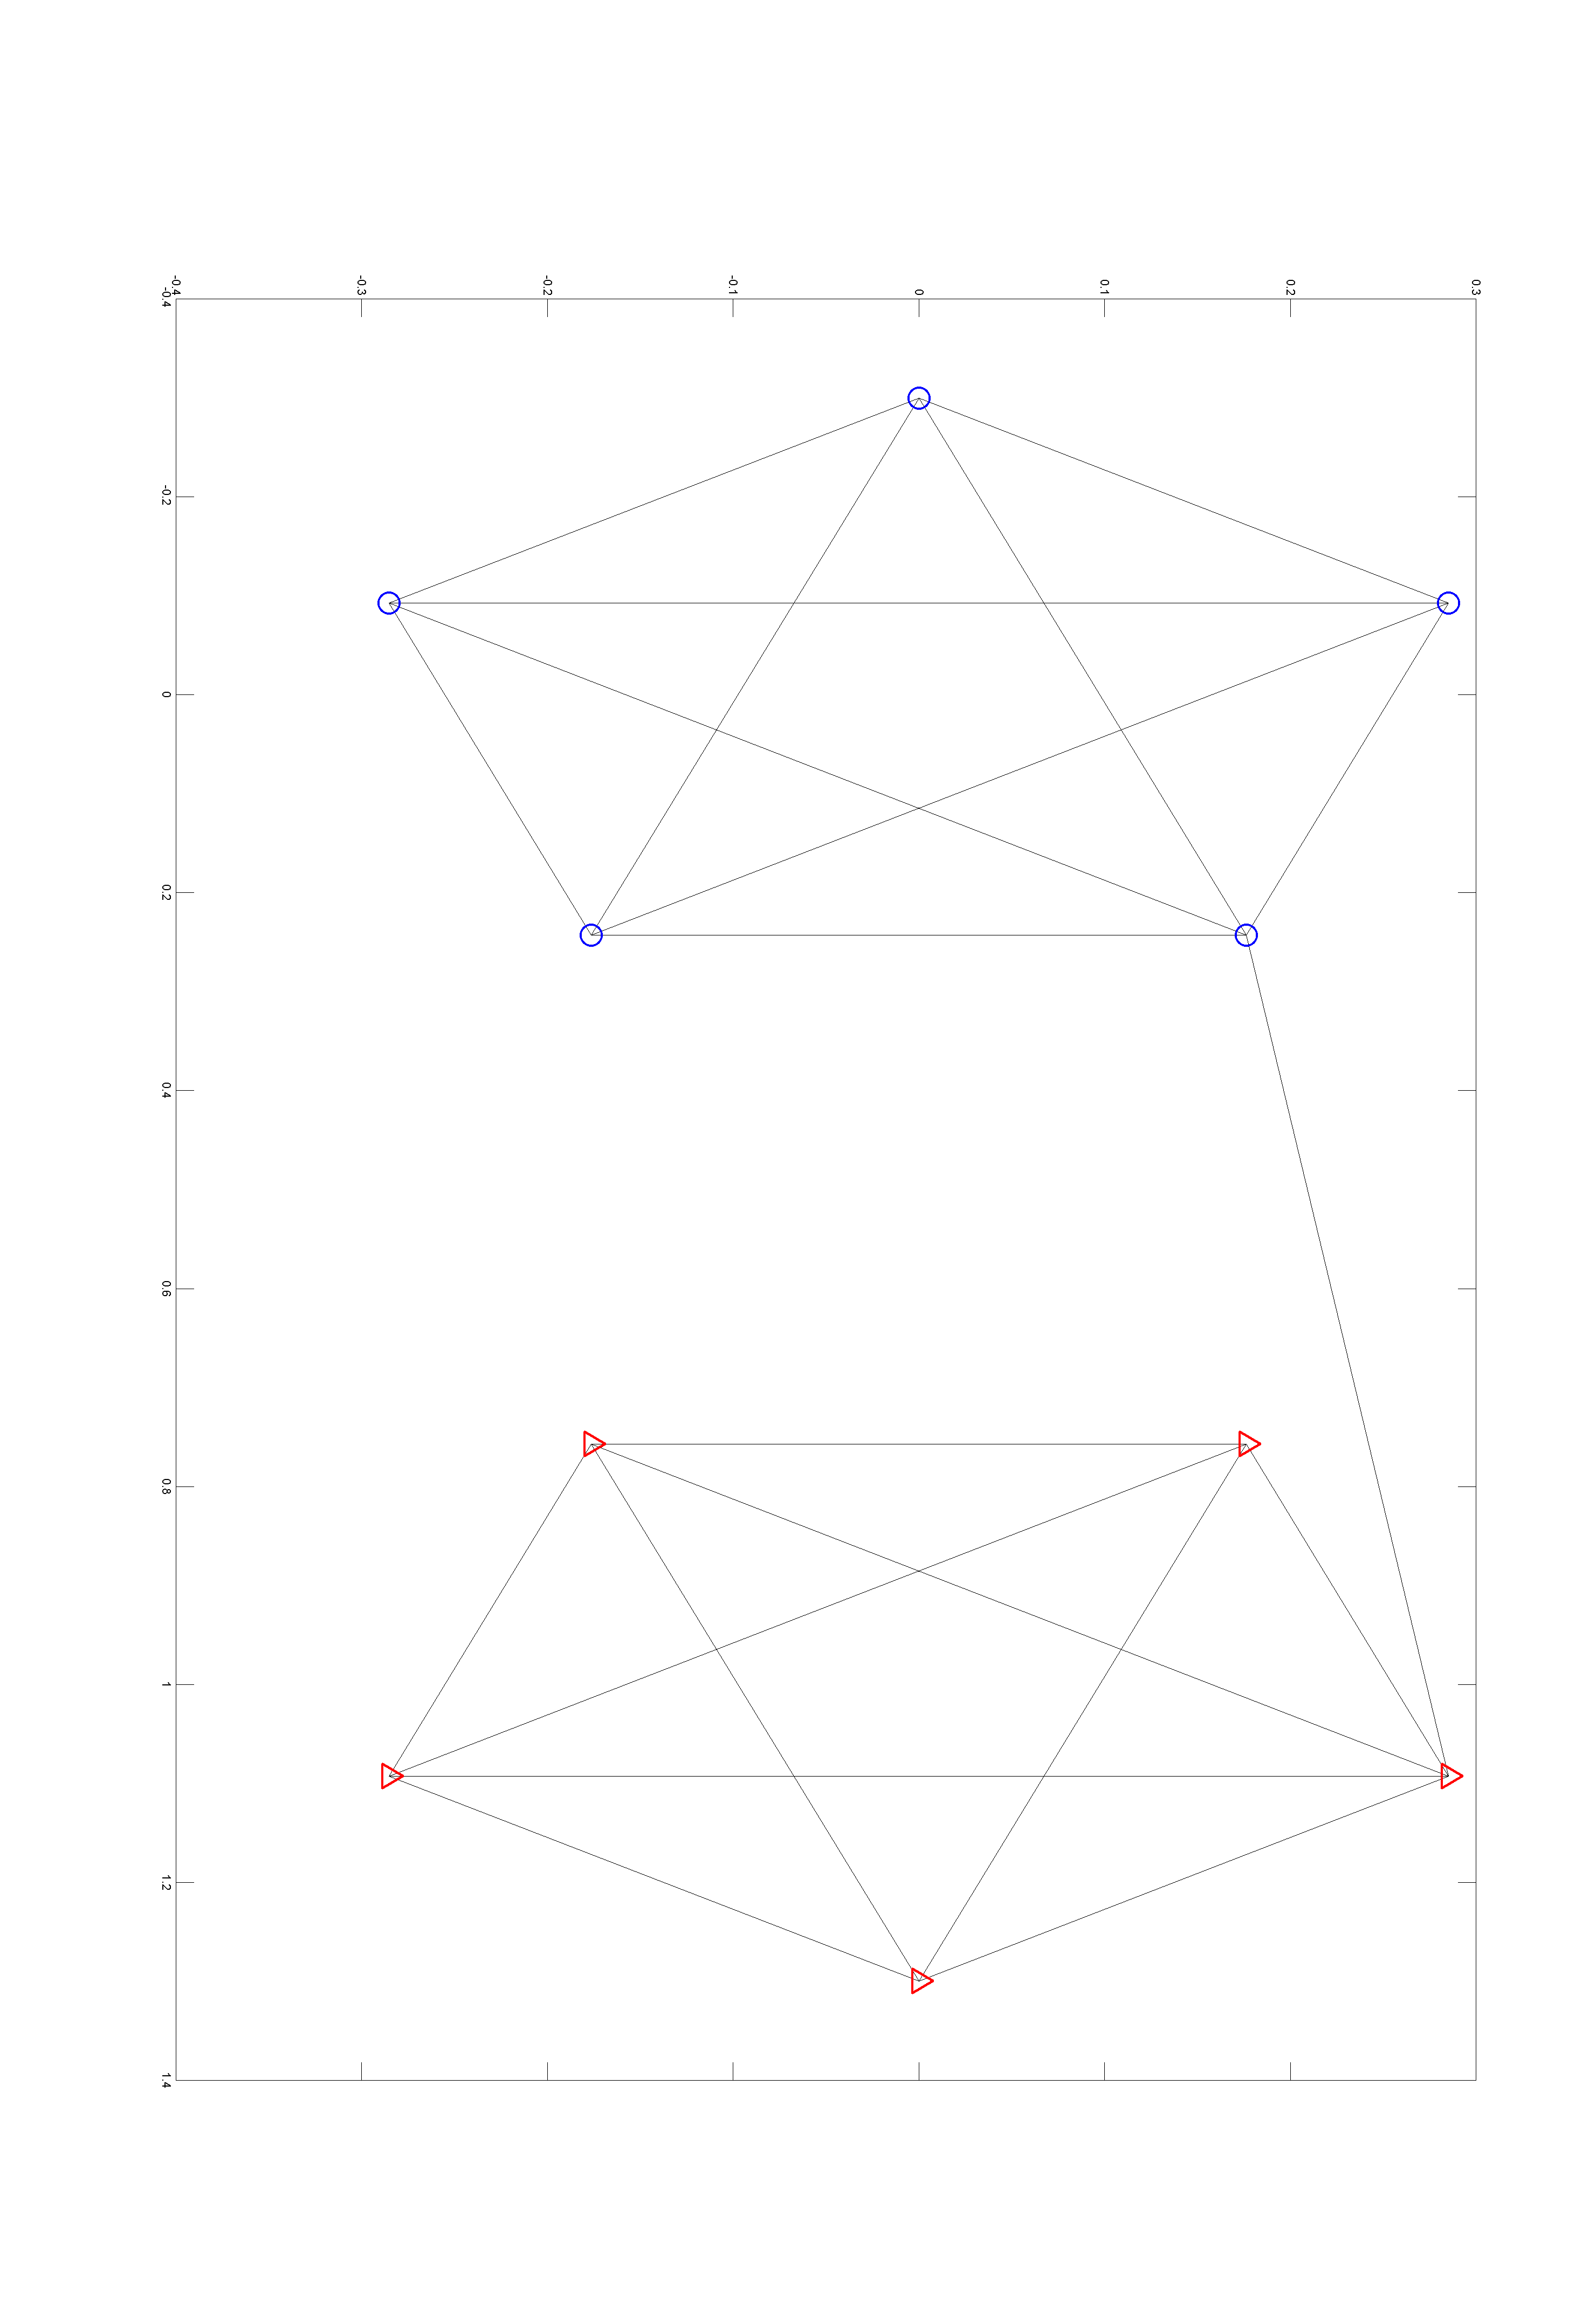
\epsfig{file = ../figures/FigNetworks-Clusters.eps,
      height=1.8cm, width=4cm, clip=, bbllx=120, bblly=260, bburx=530,
      bbury=570}  \end{tabular}
  & 2
  & $\left(\begin{array}{cc} 1&\varepsilon\\ \varepsilon&1\\
    \end{array} \right)$ &
  $\displaystyle{\frac{1+3\varepsilon^2}{(1+\varepsilon)^2}}$ \\ 
\end{tabular}
$$

% %%%%%%%%%%%%%%%%%%%%%%%%%%%%%%%%%%%%%%%%%%%%%%%%%%%%%%%%%%%%%%%%%%%%%
% \newpage
% \paragraph{Scale free network model.}
% (Barabasi \& Albert, 99)

% The network is build iteratively: the $i$-th vertex joining the
% network connects one of the $(i-1)$ preceeding ones with probability
% proportional to their current degree (\paragraph{busy gets busier}):
% $$
% \forall j < i, \qquad \Pr\vspace{0cm}^i\{ i \leftrightarrow j\} \propto K_j^i.
% $$
% The limit marginal distribution for the degrees is then scale free:
% $p(k) \propto k^{-3}$.

% \bigskip\bigskip
% \paragraph{Analogous modeling with the independent ERMG.} At time $q$,
% $n_q = n \alpha_q$ vertices join the net work. They preferentially
% connect the oldest vertices:
% $$
% \pi_{q\ell} = \eta_q \eta_{\ell}, 
% \qquad \eta_1 \geq \eta_2 \geq \dots \geq \eta_q \geq \dots 
% $$
% The decreasing speed of the $\{\eta_q\}$ gives the tail of the degree
% distribution. 

%%%%%%%%%%%%%%%%%%%%%%%%%%%%%%%%%%%%%%%%%%%%%%%%%%%%%%%%%%%%%%%%%%%%%
\newpage
\chapter{Estimation}
%%%%%%%%%%%%%%%%%%%%%%%%%%%%%%%%%%%%%%%%%%%%%%%%%%%%%%%%%%%%%%%%%%%%%

We propose to use a pseudo E-M algorithm to estimate the parameters.

%%%%%%%%%%%%%%%%%%%%%%%%%%%%%%%%%%%%%%%%%%%%%%%%%%%%%%%%%%%%%%%%%%%%%
\subsection{Likelihoods}
%%%%%%%%%%%%%%%%%%%%%%%%%%%%%%%%%%%%%%%%%%%%%%%%%%%%%%%%%%%%%%%%%%%%%

Let us denote $\Xcal = \{X_{ij}\}_{i, j = 1..n}$, $\Zcal=
\{Z_{iq}\}_{i=1..n, q=1..Q}$.

The complete-data log-likelihood is
$$
\Lcal(\Xcal, \Zcal) = \sum_i \sum_q Z_{iq} \log \alpha_q + \sum_i
\sum_q \sum_{j > i} \sum_{\ell} Z_{iq} Z_{j\ell} \log b(X_{ij};
\pi_{q\ell})
$$
where $b(x, p) = p^x (1-p)^{1-x}$.

The likelihood of the observed data is obtained by summing over all the
possible value of $\Zcal$:
$$
\exp \Lcal(\Xcal) = \sum_{\Zcal} \exp \Lcal(\Xcal, \Zcal)
$$
No simpler form has been be derived.

\newpage
The conditional expectation of the complete-data log-likelihood is:
\begin{eqnarray*}
  \Qcal(\Xcal) &=& \Esp \left\{ \Lcal(\Xcal,\Zcal)|\Xcal \right\}  \\
  \\
  &=&  \sum_i \sum_q \tau_{iq} \log \alpha_q
  + \sum_i \sum_q \sum_{j > i} \sum_{\ell} \theta_{ijq\ell} \log
  b(X_{ij}; \pi_{q\ell}),
\end{eqnarray*}
where
\begin{eqnarray*}
\tau_{iq} & = & \Pr\{Z_{iq} = 1 \;|\; \Xcal\} = \Esp(Z_{iq} \;|\;
\Xcal), \\
\\
\theta_{ijq\ell} & = & \Pr\{Z_{iq} Z_{j\ell} = 1 \;|\; \Xcal\} =
\Esp(Z_{iq} Z_{j\ell} \;|\; \Xcal). 
\end{eqnarray*}
% These \textit{posterior} probabilities satisfy
% $$
%   \sum_q  \tau_{iq} = 1, \qquad
%   \theta_{ijq\ell} = \theta_{ji\ell q}, \qquad
%   \sum_q \sum_{\ell} \theta_{ijq\ell} = 1, \qquad
%   \tau_{iq} = \sum_{\ell} \theta_{ijq\ell}.
% $$
These \textit{posterior} probabilities are difficult to caculate and
need to be 
\begin{itemize}
\item \vspace{-0.5cm} either approximated ('mean field' approximation) 
\item \vspace{-0.5cm} or estimated (Gibbs sampling, MCMC).
\end{itemize}

% %%%%%%%%%%%%%%%%%%%%%%%%%%%%%%%%%%%%%%%%%%%%%%%%%%%%%%%%%%%%%%%%%%%%%
% \newpage
% \subsection{Approximation of the $\theta_{ijq\ell}$}
% %%%%%%%%%%%%%%%%%%%%%%%%%%%%%%%%%%%%%%%%%%%%%%%%%%%%%%%%%%%%%%%%%%%%%
% \begin{itemize}
% \item $\theta_{ijq\ell}$ turns out to be difficult to evaluate.
% \item Conditional independence used to simplify such calculations in
%   Hidden Markov Field do not hold here since the neighborhood of each
%   vertex is the whole graph.
% \end{itemize}

% \paragraph{Additional conditioning.} We propose to approximate $\theta_{ijq\ell}$ by
% $$
% \theta_{ijq\ell} \simeq \Pr\{Z_{iq} Z_{j\ell} = 1 \;|\; \Xcal,
% \Zcal^{ij}\} \propto \Pr\{Z_{iq} Z_{j\ell} = 1, \Xcal \;|\;
% \Zcal^{ij}\}.
% $$
% This last quantity is easier to calculate:
% $$
% \Pr\{Z_{iq} Z_{j\ell} = 1, \Xcal \;|\; \Zcal^{ij}\} \propto
% \alpha_q \alpha_{\ell} b(X_{ij}, \pi_{q\ell}) \prod_{m} b(C^j_{im};
% N^{ij}_{m} , \pi_{qm}) b(C^i_{jm}; N^{ij}_{m}, \pi_{\ell m})
% $$
% where $N_m = \sum_{k \neq i, j} Z_{km}$ and $C_{im} = \sum_{k \neq
%   j} Z_{km} X_{ik}$.

% %%%%%%%%%%%%%%%%%%%%%%%%%%%%%%%%%%%%%%%%%%%%%%%%%%%%%%%%%%%%%%%%%%%%%
% \newpage
% \paragraph{Mean field approximation.}
% The preceding approximation can not be used as such since
% $\Zcal^{ij}$ is unknown.

% Several prediction methods can be considered:
% $$
% \begin{tabular}{lll} 
%   MAP: & $\widehat{Z}_{iq} = \Ibb\{\arg\max_{\ell}\tau_{i\ell}\}$
%   & (Classification EM). \\
%   \\
%   Random assignment: & $(\widehat{Z}_{i1}, .\, .\, \widehat{Z}_{iQ})
%   \sim \Mcal(1; \tau_{i1},\,.\,. \tau_{iQ})$
%   & (Stochastic EM). \\
%   \\
%   Posterior probability: & $\widehat{Z}_{iq} = \tau_{iq}$ & (standard
%   EM).
% \end{tabular}
% $$
% In practice, the latter seems to perform better.

% \bigskip
% The approximation of $\theta_{ijq\ell}$ is obtained by plugging
% $\widehat{Z}_{iq}$ into $N_m$ and $C_{im}$:
% $$
% \widehat{\theta}_{ijq\ell} \propto \alpha_q \alpha_{\ell}
% b(X_{ij}, \pi_{q\ell}) \prod_{m} b(\widehat{C}^j_{im};
% \widehat{N}^{ij}_{m} , \pi_{qm}) b(\widehat{C}^i_{jm};
% \widehat{N}^{ij}_{m}, \pi_{\ell m})
% $$

% %%%%%%%%%%%%%%%%%%%%%%%%%%%%%%%%%%%%%%%%%%%%%%%%%%%%%%%%%%%%%%%%%%%%%
% \newpage
% \paragraph{Alternative way: Gibbs sampling.}
% \begin{itemize}
% \item The conditional distribution of $Z_i$ given $\Zcal^i$ can be
%   easily simulated:
%   $$
%   \Pr\{Z_{iq} = 1 \;|\; \Xcal, \Zcal^i\} \propto \alpha_q \prod_{m}
%   b(C_{im}; N^{i}_{m} , \pi_{qm}).
%   $$
% \item Denoting $ \Zcal^{(h)} = \{Z_i^{(h)}\}_i$ at step $h$, the joint
%   distribution of the $Z_i^{(h+1)}$:
%   $$
%   Z_i^{(h+1)} \sim \Pr\{ Z_i \;|\; \Xcal, \Zcal^{i, (h)}\},
%   $$
%   tends to the joint conditional distribution of the $\{Z_i \;|\;
%   \Xcal\}_i$.
% \item Performing a 'large' number $H$ of simulations (after some burning
%   time), we get
%   $$
%   \widehat{\tau}_{iq} = \frac1H \sum_h Z_{iq}^{(h)}, 
%   \qquad
%   \widehat{\theta}_{ijq\ell} = \frac1H \sum_h Z_{iq}^{(h)} Z_{j\ell}^{(h)}. 
%   $$
% \end{itemize}

%%%%%%%%%%%%%%%%%%%%%%%%%%%%%%%%%%%%%%%%%%%%%%%%%%%%%%%%%%%%%%%%%%%%%
\newpage
\subsection{Pseudo E-M algorithm}
%%%%%%%%%%%%%%%%%%%%%%%%%%%%%%%%%%%%%%%%%%%%%%%%%%%%%%%%%%%%%%%%%%%%%

\paragraph{Pseudo E step.}
Since equation $\tau_{iq} = \sum_{\ell} \theta_{ijq\ell}$ is true for
all $j$, we estimate $\tau_{iq}$ with a simple average over all the
possible $j$s:
$$
\widehat{\tau}_{iq} = \sum_{j \neq i} \sum_{\ell}
\widehat{\theta}_{ijq\ell} \left/ (n-1) \right..
$$

\paragraph{M step.}
At this step, we maximize the function $\Qcal(\Xcal)$ subject to
$\sum_q \alpha_q = 1$. 

We get
$$
\widehat{\alpha}_q = \sum_i \widehat{\tau}_{iq} / n, \qquad
\widehat{\pi}_{q\ell} = \sum_i \sum_j \widehat{\theta}_{ijq\ell}
X_{ij} \left/ \sum_i \sum_j \widehat{\theta}_{ijq\ell} \right..
$$

%%%%%%%%%%%%%%%%%%%%%%%%%%%%%%%%%%%%%%%%%%%%%%%%%%%%%%%%%%%%%%%%%%%%%
\newpage
\subsection{Choice of the number of groups}
%%%%%%%%%%%%%%%%%%%%%%%%%%%%%%%%%%%%%%%%%%%%%%%%%%%%%%%%%%%%%%%%%%%%%

We propose a heuristic penalized likelihood criterion inspired from
BIC.
% We propose a heuristic criterion inspired from the Integrated
% Completed Likelihood (ICL, Biernacki et al., 2000) which applies the
% same penalty as BIC to the complete-data log-likelihood (only
% available here).

$\Qcal(\Xcal)$ is the sum of
$$
\begin{tabular}{p{11cm}p{13cm}}
  $\displaystyle{\sum_i \sum_q \tau_{iq} \log \alpha_q}$ & 
  which deals with $(Q-1)$ independent proportions $\alpha_q$s and
  involves $n$ data 
  \\ 
  \\
  $\displaystyle{\sum_i \sum_q \sum_{j > i} \sum_{\ell} \theta_{ijq\ell} \log
    b(X_{ij}; \pi_{q\ell})}$ 
  & which deals with $Q(Q+1)/2$ probabilities $\pi_{q\ell}$s and
  involves $n(n-1)/2$ terms. 
\end{tabular}
$$
We propose the following heuristic criterion:
$$
  - 2\Qcal(\Xcal) + (Q-1) \log n + Q(Q+1)/2 \log[n(n-1)/2].
$$

%%%%%%%%%%%%%%%%%%%%%%%%%%%%%%%%%%%%%%%%%%%%%%%%%%%%%%%%%%%%%%%%%%%%%
\newpage
\chapter{Application to {\it E. coli} reaction network}
%%%%%%%%%%%%%%%%%%%%%%%%%%%%%%%%%%%%%%%%%%%%%%%%%%%%%%%%%%%%%%%%%%%%%

Fit of the ERMG model to a graph with $n=605$ vertices and $1\;782$
edges.

\paragraph{Choice of the number of groups.}
\vspace{-0.5cm}
$$
  \begin{tabular}{l}
    {\bf ---}: log-likelihood $\Qcal$ \\
    \\ \\
    \textblue{\bf - -}: heuristic criterion \\
    \\ \\
    \textred{$\bf \cdots$}: maximum at $Q = 6$
  \end{tabular}
  \begin{tabular}{c}
    \epsfig{file = ../figures/FigEColi-LcBIC.eps, height=12cm, width=12cm, clip=}
  \end{tabular}
$$ 

\newpage
\paragraph{Parameter estimates.}
$$
\begin{array}{ccccccc}
  q & 1 & 2 & 3 & 4 & 5 & 6 \\
  \hline
  \widehat{\alpha} (\%) & 2.3 & 3.0 & 3.5  & 22.9  & 30.2  & 38.2 \\
  \hline
  & 100  & \varepsilon & 0.6 & 1.3 & \varepsilon & 0.5 \\
  & \varepsilon & 100  & \varepsilon & 0.5 & 0.2 & 0.9 \\
  \widehat{\pi}_{q\ell}  & 0.6 & \varepsilon & 100  & 3.0 & 0.2 & 0.4 \\
  (\%) & 1.3 & 0.5 & 3.0 & 5.0 & 0.3 & 0.1 \\
  & \varepsilon & 0.2 & 0.2 & 0.3 & 1.6 & 0.1 \\
  & 0.5 & 0.9 & 0.4 & 0.1 & 0.1 & 0.9 \\
  \hline
  \widehat{\lambda}_q & 17.1 &  21.1 & 26.5 & 8.5 & 3.7 & 2.6 \\
\end{array}
$$

The first three groups are actually three cliques of size 14, 18 and 21.

No connection exists between the first two cliques. 

Vertices from group 3 have rather frequent connections with group 4.

The clique structure strongly increases the mean degree $\lambda_q$ of
its elements.

\newpage
%~\vspace{-3cm}
%$$
\hspace{-2cm}
\begin{tabular}{cc}
  \begin{tabular}{p{11cm}}
    \paragraph{Dot-plot representation of the graph.} \\ \\
    Dot present means 
    $$X_{ij} = 1$$
    The vertices are re-ordered according to their 'mean group
    number':
    $$
    \widehat{q}_i = \sum_q q \; \widehat{\tau}_{iq} 
    $$
  \end{tabular}
  &
  \begin{tabular}{c}
    \epsfig{file = ../figures/FigEColi-ERMG.eps, height=12cm,
      width=12cm, clip=,bbllx=70, bblly=440, bburx=540, bbury=720}  
  \end{tabular} \\
  \begin{tabular}{p{11cm}}
    \paragraph{Posterior probabilities $\widehat{\tau}_{iq}$.}  \\ \\ \\
  \end{tabular}
  & 
  \begin{tabular}{c}
    \epsfig{file = ../figures/FigEColi-ERMG.eps, width=12cm, clip=,
      bbllx=70, bblly=250, bburx=540, bbury=400} 
  \end{tabular}
\end{tabular}
%$$

\newpage
\paragraph{Between group connectivity.} \\
Top right = 'observed' connectivities $A_{q\ell}$ (bottom left = expected)
$$
\begin{tabular}{ccccccc}
  Group & 1 & 2 & 3 & 4 & 5 & 6 \\
  \hline
  1 & 98~(91) &    0 &    1 &   13 &    0 &    8 \\
  2 & (0) &  162~(153) &    0 &    6 &    3 &   18 \\
  3 & (2) &    (0) &  220~(210) &   44 &    4 &    9 \\
  4 & (12) &    (6) &   (47) &  475~(477) &   42 &    8 \\
  5 & (0) &    (4) &    (5) &   (40) &  268~(268) &   20 \\
  6 & (8) &   (18) &    (9) &    (9) &   (18) &  230~(235) \\
\end{tabular}
$$
but the observed $A_{q\ell}$ are unobserved and estimated with the MAP
rule:
$$
{\widehat{A}_{q\ell} = \sum_{i<j} \widehat{Z}_{iq}
  \widehat{Z}_{j\ell} X_{ij}} \quad \Rightarrow \quad \mbox{the
  good observed fit is optimistic.}
$$
\paragraph{Clustering coefficient.}
$$
\begin{tabular}{cccc}
  Empirical & ERMG ($Q = 6$) & ERMG ($Q = 4$) & ER \\
  \hline
  0.626 & 0.455 & 0.474 & 0.0098
\end{tabular}
$$

%%%%%%%%%%%%%%%%%%%%%%%%%%%%%%%%%%%%%%%%%%%%%%%%%%%%%%%%%%%%%%%%%%%%%%%%
\newpage
\chapter{Conclusions}

\paragraph{Past.} 
\begin{itemize}
\item \vspace{-0.5cm} The ERMG model is a flexible generalization of
  the ER model and a promising alternative to the scale-free 'model'.
\item \vspace{-0.5cm} It seems to fit well several real-world networks
  %(Airport network, Enzyme network in bacterias, etc.).
\item \vspace{-0.5cm} It is properly defined, so its properties can be
  properly studied.
\end{itemize}

\paragraph{Future.}
\begin{itemize}
\item \vspace{-0.5cm} Study the probabilistic properties of the ERMG
  model (diameter, probability for a subgraph to be connected, etc).
\item \vspace{-0.5cm} Derive the statistical properties of the
  proposed algorithm or propose a new estimation algorithm.
\item \vspace{-0.5cm} Derive a relevant criterion to select the number
  of groups.
\item \vspace{-0.5cm} Extension to valued graphs: $X_{ij}$ not only
  0/1, but some measure of the connexion.
\end{itemize}

%%%%%%%%%%%%%%%%%%%%%%%%%%%%%%%%%%%%%%%%%%%%%%%%%%%%%%%%%%%%%%%%%%%%%%%%
%%%%%%%%%%%%%%%%%%%%%%%%%%%%%%%%%%%%%%%%%%%%%%%%%%%%%%%%%%%%%%%%%%%%%%%%
%%%%%%%%%%%%%%%%%%%%%%%%%%%%%%%%%%%%%%%%%%%%%%%%%%%%%%%%%%%%%%%%%%%%%%%%
%%%%%%%%%%%%%%%%%%%%%%%%%%%%%%%%%%%%%%%%%%%%%%%%%%%%%%%%%%%%%%%%%%%%%%%%
\end{document}
%%%%%%%%%%%%%%%%%%%%%%%%%%%%%%%%%%%%%%%%%%%%%%%%%%%%%%%%%%%%%%%%%%%%%%%%
%%%%%%%%%%%%%%%%%%%%%%%%%%%%%%%%%%%%%%%%%%%%%%%%%%%%%%%%%%%%%%%%%%%%%%%%
%%%%%%%%%%%%%%%%%%%%%%%%%%%%%%%%%%%%%%%%%%%%%%%%%%%%%%%%%%%%%%%%%%%%%%%%
%%%%%%%%%%%%%%%%%%%%%%%%%%%%%%%%%%%%%%%%%%%%%%%%%%%%%%%%%%%%%%%%%%%%%%%%

